\section{Cross-Site Request Forgery (CSRF)}
CSRF is an attack that forces an end user to execute unwanted actions on a web application in which they're currently authenticated. This attacks have two parts. First the attacker must design the URL or script, then trick the victim into activating it via social engineering or camouflage of the URL. If the web application is badly designed and state changes can be made through GET requests, the attacker can design a URL such as

\begin{verbatim}
	http://bank.com/transfer.do?acct=MARIA&amount=100000
\end{verbatim}
When the victim's browser makes a request to this site, automatically sends the correct cookies with it, and the web application makes the transfer. There are several ways to trick the victim into sending this petition, like disguising it as a fake link: 

\begin{verbatim}
<a href="http://bank.com/transfer.do?acct=MARIA&amount=100000">
View my Pictures!</a>
\end{verbatim}
Or tag it as a image, so the request is automatically made when the page loads:
\begin{verbatim}
<img src="http://bank.com/transfer.do?acct=MARIA&amount=100000" width="0" 
height="0" border="0">
\end{verbatim} 
The obvious solution to this problem seems to be to redesign the web application correctly, so that requests that change something are made with a POST instead of a GET, like the HTTP standard suggests. This should be done, but the application still would not be secure.

\subsection{POST request attack}
Now imagine that we redesign the application so that state-changing requests are POST. Now a correct requests looks like this:
\begin{verbatim}
POST http://bank.com/transfer.do HTTP/1.1

acct=BOB&amount=100
\end{verbatim}
This request cannot be made with a simple link, but still can be generated using a disguised form:

\begin{verbatim}
<form action="<nowiki>http://bank.com/transfer.do</nowiki>" method="POST">
<input type="hidden" name="acct" value="MARIA"/>
<input type="hidden" name="amount" value="100000"/>
<input type="submit" value="View my pictures"/>
</form>
\end{verbatim}
When the user clicks what he suspects is a link, a form request genereates a POST that sends the values. This can be further improved with adding this js line in the html, that sends the form automatically when the user loads the page.

\begin{verbatim}
<body onload="document.forms[0].submit()">
\end{verbatim}

\subsection{CSRF Prevention}
There are two steps in CSRF protection. Check origin and CSRF token.
%https://developer.mozilla.org/en-US/docs/Glossary/Forbidden_header_name
\subsubsection{Check origin}
To identify the source, we can check one of this HTTP headers, Origin Header and Referer Header.
The Origin Header is one of the Headers that cannot be edited by the js running in the browser. It can only be created and modified by the browser, so if we are assuming the victim's browser is safe, the header can be trusted. If this header is present, it should be checked to make sure it matches the destination. Acording to https://wiki.mozilla.org/Security/Origin, Origin headers are included when the request is originated inside an iframe, a form or through js.If there's no Origin header, then we should check the referer header. The referer identifies the adress of the webpage that linked to the source being requested. If there aren't any of this headers, the recommended thing to do is to reject the request.
\subsubsection{CSRF token}
The CSRF token consists of a secure random token that is generated with each session. The token is sent with the html forms generated by the website as a hidden field. When the web app recieves a request it checks the token to match the session token. This way, only a form generated by the web application can know the token and be valid.

\subsection{Same origin policy}
Same origin policy is used by the browser to allow \textbf{scripts} in webpage A to make requests to webpage B but only if A and B have the same origin.
This tries to protect the user from malicious website A having scripts that request data from safe website B using the user's cookies and session. For the browser to allow a request from a script, the request must be sent using the same protocol (\verb|http| and \verb|https| are different), the same port number and exactly the same domain (\verb|subdomain.domain.com| and \verb|domain.com| won't work).

\section{Cross-origin Resource Sharing (CORS)}
Sometimes we need to access resources from other servers, and make exceptions to the same origin policy. This is accomplished differently depending on the request type.

\subsection{GET}
 % Perquè es el browser el encarregat de fer reject de les peticions? el interesat es el propi server. Perque el servidor no fa el block? Pq fa la resposta i confia en el client?
A GET request should not change the state of anything in the web application, only return content. 
Imagine we are browsing a website called \verb|somesite.com|, and this web has js code that requests data from \verb|mybank.com|. First, the code in the browser makes the GET request to the content of the \verb|mybank.com|. The browser sets the headers as \verb|Origin: bad.com| and sends it. If the server wants to allow \verb|somesite.com| to acess this data, the server then generates the response, and sends it with the header \verb|Access-Control-Allow-Origin: somesite.com|. This tells the browser that the server allows the code to access the data. The header can also be set as \verb|Acess-Control-Allow-Origin: *|, so that any website is valid. It's very important to understand that the browser blocks the response from the server, not the request.

\begin{figure}[htb]
	\begin{centering}
		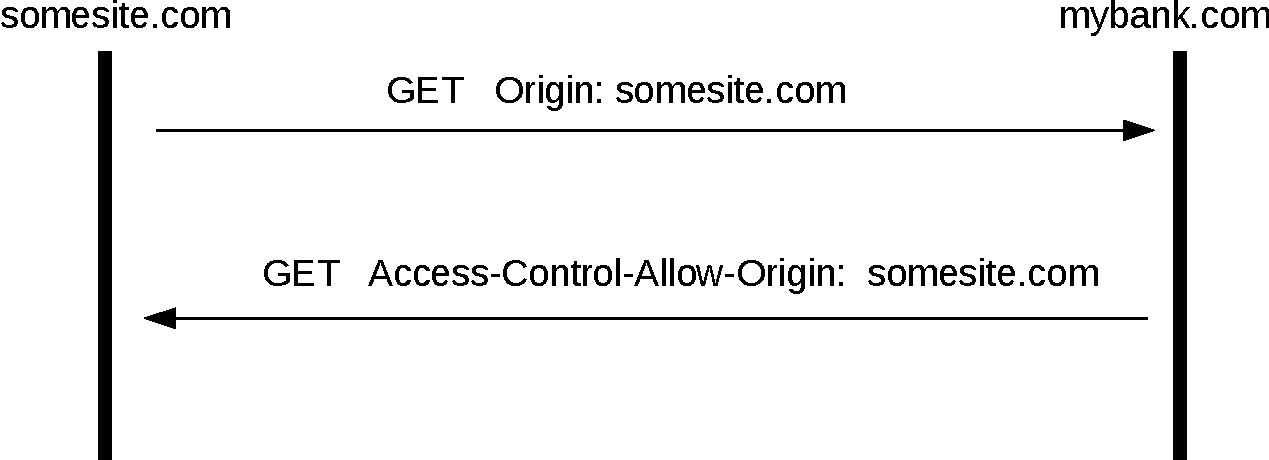
\includegraphics[width=0.7\columnwidth]{\securitydir/WebSec/figures/cors-get}
		\par\end{centering}
	\caption{\label{fig:ecb} Diagram of a CORS GET request.}
\end{figure}


\subsection{Pre-flight requests}
POST, PUT, DELETE requests should change the state, or modify the DB. This means that if we use the same technique as the GET, when the browser blocks the response, the changes in the server are already made and it's too late to block it. For this reason, we use a \textbf{pre-flight request}. When the browser detects that code wants to make a request that modifies state (for example a POST) to another website, first it sends a OPTIONS request, with the header \texttt{Acess-Control-Request-Method: POST}. If the server accepts this kind of request from this website, has to respond with the headers \verb|Acess-Control-Allow-Origin: somesite.com| and  \texttt{Acess-Control-Allow
-Methods: POST}. Doing this the browser knows that \verb|mybank.com| allows requests from this sites with the methods shown. Then the browser makes the real request, with the same header \verb|Origin: somesite.com|. 


\begin{figure}[htb]
	\begin{centering}
		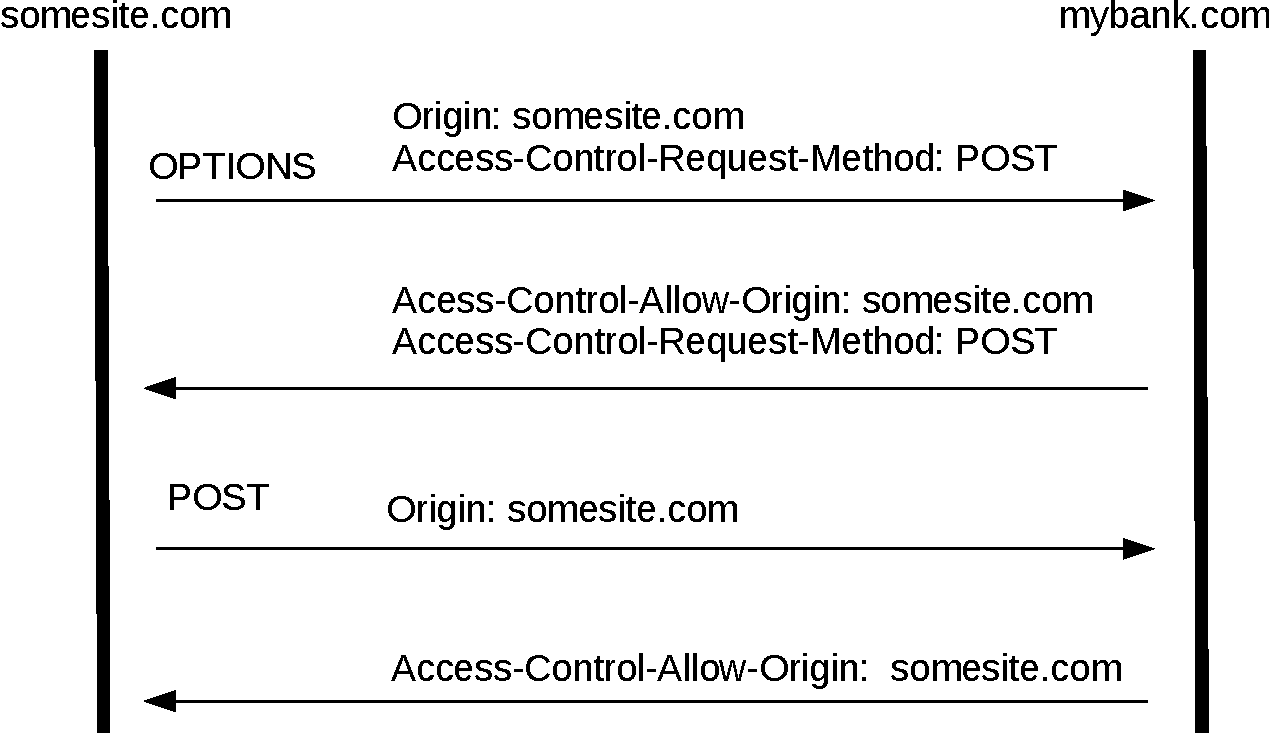
\includegraphics[width=0.7\columnwidth]{\securitydir/WebSec/figures/cors-post}
		\par\end{centering}
	\caption{\label{fig:ecb} Diagram of a CORS POST request with a pre-flight.}
\end{figure}